\section{CD Pipeline Implementation [Rahat Rafiq]}\label{sec:cd_pipeline_implementaiton}

Azure CD pipeline will also have just one agent job consisting of a few tasks. CD pipeline is configured independently of the CI pipeline. Only in the event of a push event to a specific azure container registry, the CD pipeline will become active. In the implemented solution there will be two CD pipeline solutions. One pipeline for staging environment and another for production. 

\subsection{Configuring CD Pipeline Triggers and Artifacts}
As discussed in the previous sections, there will be two release pipelines, thus there will be two separate triggers. Both of these triggers have to be configured for a specific repository push of events of two different azure container registries. Azure DevOps provides an intuitive UI for configuring release triggers. First, the list of necessary artifacts has to be added to the release pipeline. The artifacts that were packaged and dropped in the azure artifacts directory from a subsequent CI build have to be added in the CD pipeline, then the azure container registry repositories where the CI pipeline pushes the application images have to be added as artifacts. Then the necessary continuous deployment triggers can be easily set up for these added artifact repositories. ~\ref{fig:cd_pipeline_trigger_and_artifacts}

\begin{figure}
    \centering
    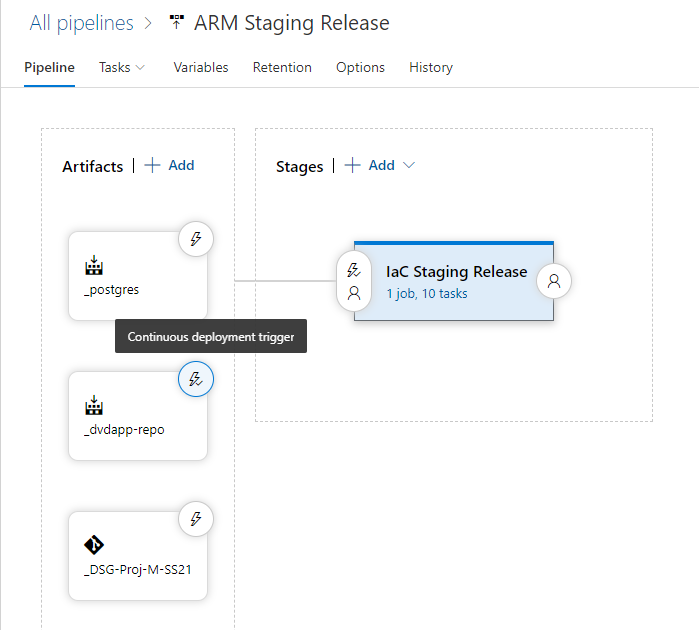
\includegraphics[width=14cm]{images/Rahat/cd-trigger.png}
    \caption{CD Pipeline Trigger and Artifacts}
    \label{fig:cd_pipeline_trigger_and_artifacts}
\end{figure}

The following subsections discuss the tasks of the implemented CD pipeline solution of the spring boot application in detail:

\subsection{Pull Artifacts}
The first task of the agent job is to pull the artifacts that were defined for the pipeline in the previous step. It is important to note that this artifact pull event occurs specifically for the corresponding CI build. Each CI build has a build ID that facilitates this mechanism. It ensures that at all times the latest corresponding artifacts are pulled from the directory, thus avoiding the usage of a previous version of artifacts. 

\subsection{ARM Template Deployment}
This job implements the whole Infrastructure as code (IaC) architecture of the implementation. Azure Resource Manager or ARM is the in-house solution for IaC provided by Microsoft and azure and has the best integration with the azure virtual cloud. This task will utilize two JSON ARM scripts that were made available to the release pipeline through azure artifacts and dynamically provision an Azure Kubernetes Service (AKS) cluster to the specified Resource group of the azure portal. This ARM deployment will also ensure the dynamic load-balancing capabilities of AKS cluster node machines. This ARM task and the load-balancing architecture are discussed in detail in the Infrastructure as Code (IaC) section. ~\ref{sec:infrastructure_as_code}

\subsection{Set AKS Context}
Similar to the CI pipeline the CD pipeline is also executed in a Microsoft hosted VM. This virtual machine has access to the Azure portal through a service principal account. However, before deploying the application it is necessary to set the correct Kubernetes context in the hosted machine. To achieve this in self-hosted Kubernetes clusters, it was necessary to edit the Kube-config configuration file located in the cluster file directory but it has been made easier in the Azure cloud environment. In azure, a simple az module command using Azure CLI can set the right context for deployment. The hosted VM provided by azure already comes with az module CLI pre-installed. This step only specifies am azure CLI task that executes that command in the hosted VM. 

\subsection{Create and Destroy Image-pull Secrets}
Azure container registry is a private image repository. Thus it is necessary to provide registry credentials each time the CD pipeline pulls an image from ACR. Since the target deployment environment for the application is Kubernetes, the best way to handle the ACR credential is to a create Kubernetes secret. This step of the job will create a Kubernetes secret with ACR admin credentials. However, it is essential to prune this secret after a successful deployment of the application for security purposes. That's why this secret will be deleted through another task after the next two tasks of the agent job are successfully executed. 

\subsection{Create Kubernetes Deployment Objects}
In a previous task, the ARM template has provisioned the AKS cluster and set up the basic AKS node pool load-balancing. This step will deploy the application and the database in the AKS cluster. The necessary Kubernetes deployment manifests were already pulled from the artifacts directory. This task will run kubectl apply command on those manifest files and create a dvdstore and PostgreSQL deployment objects.

\subsection{Create Kubernetes Service Objects}
This is the last task of the CD pipeline. In this task, the pipeline will run the kubectl apply command on two service objects. One service object will expose the dvdstore application deployment on a specific HTTP port with a load balancer and another object will expose the PostgreSQL deployment as a ClusterIP, so it is available to open connections to the dvdstore application service.





